\chapter{Будова та функція печінки}

\section{Що таке печінка?}

Печінка - це найбільший орган черевної порожнини, «біохімічна лабораторія» організму, яка виконує велику кількість життєво важливих для людини функцій (Мал. \ref{fig:healthyliver}).



\begin{marginfigure}%
  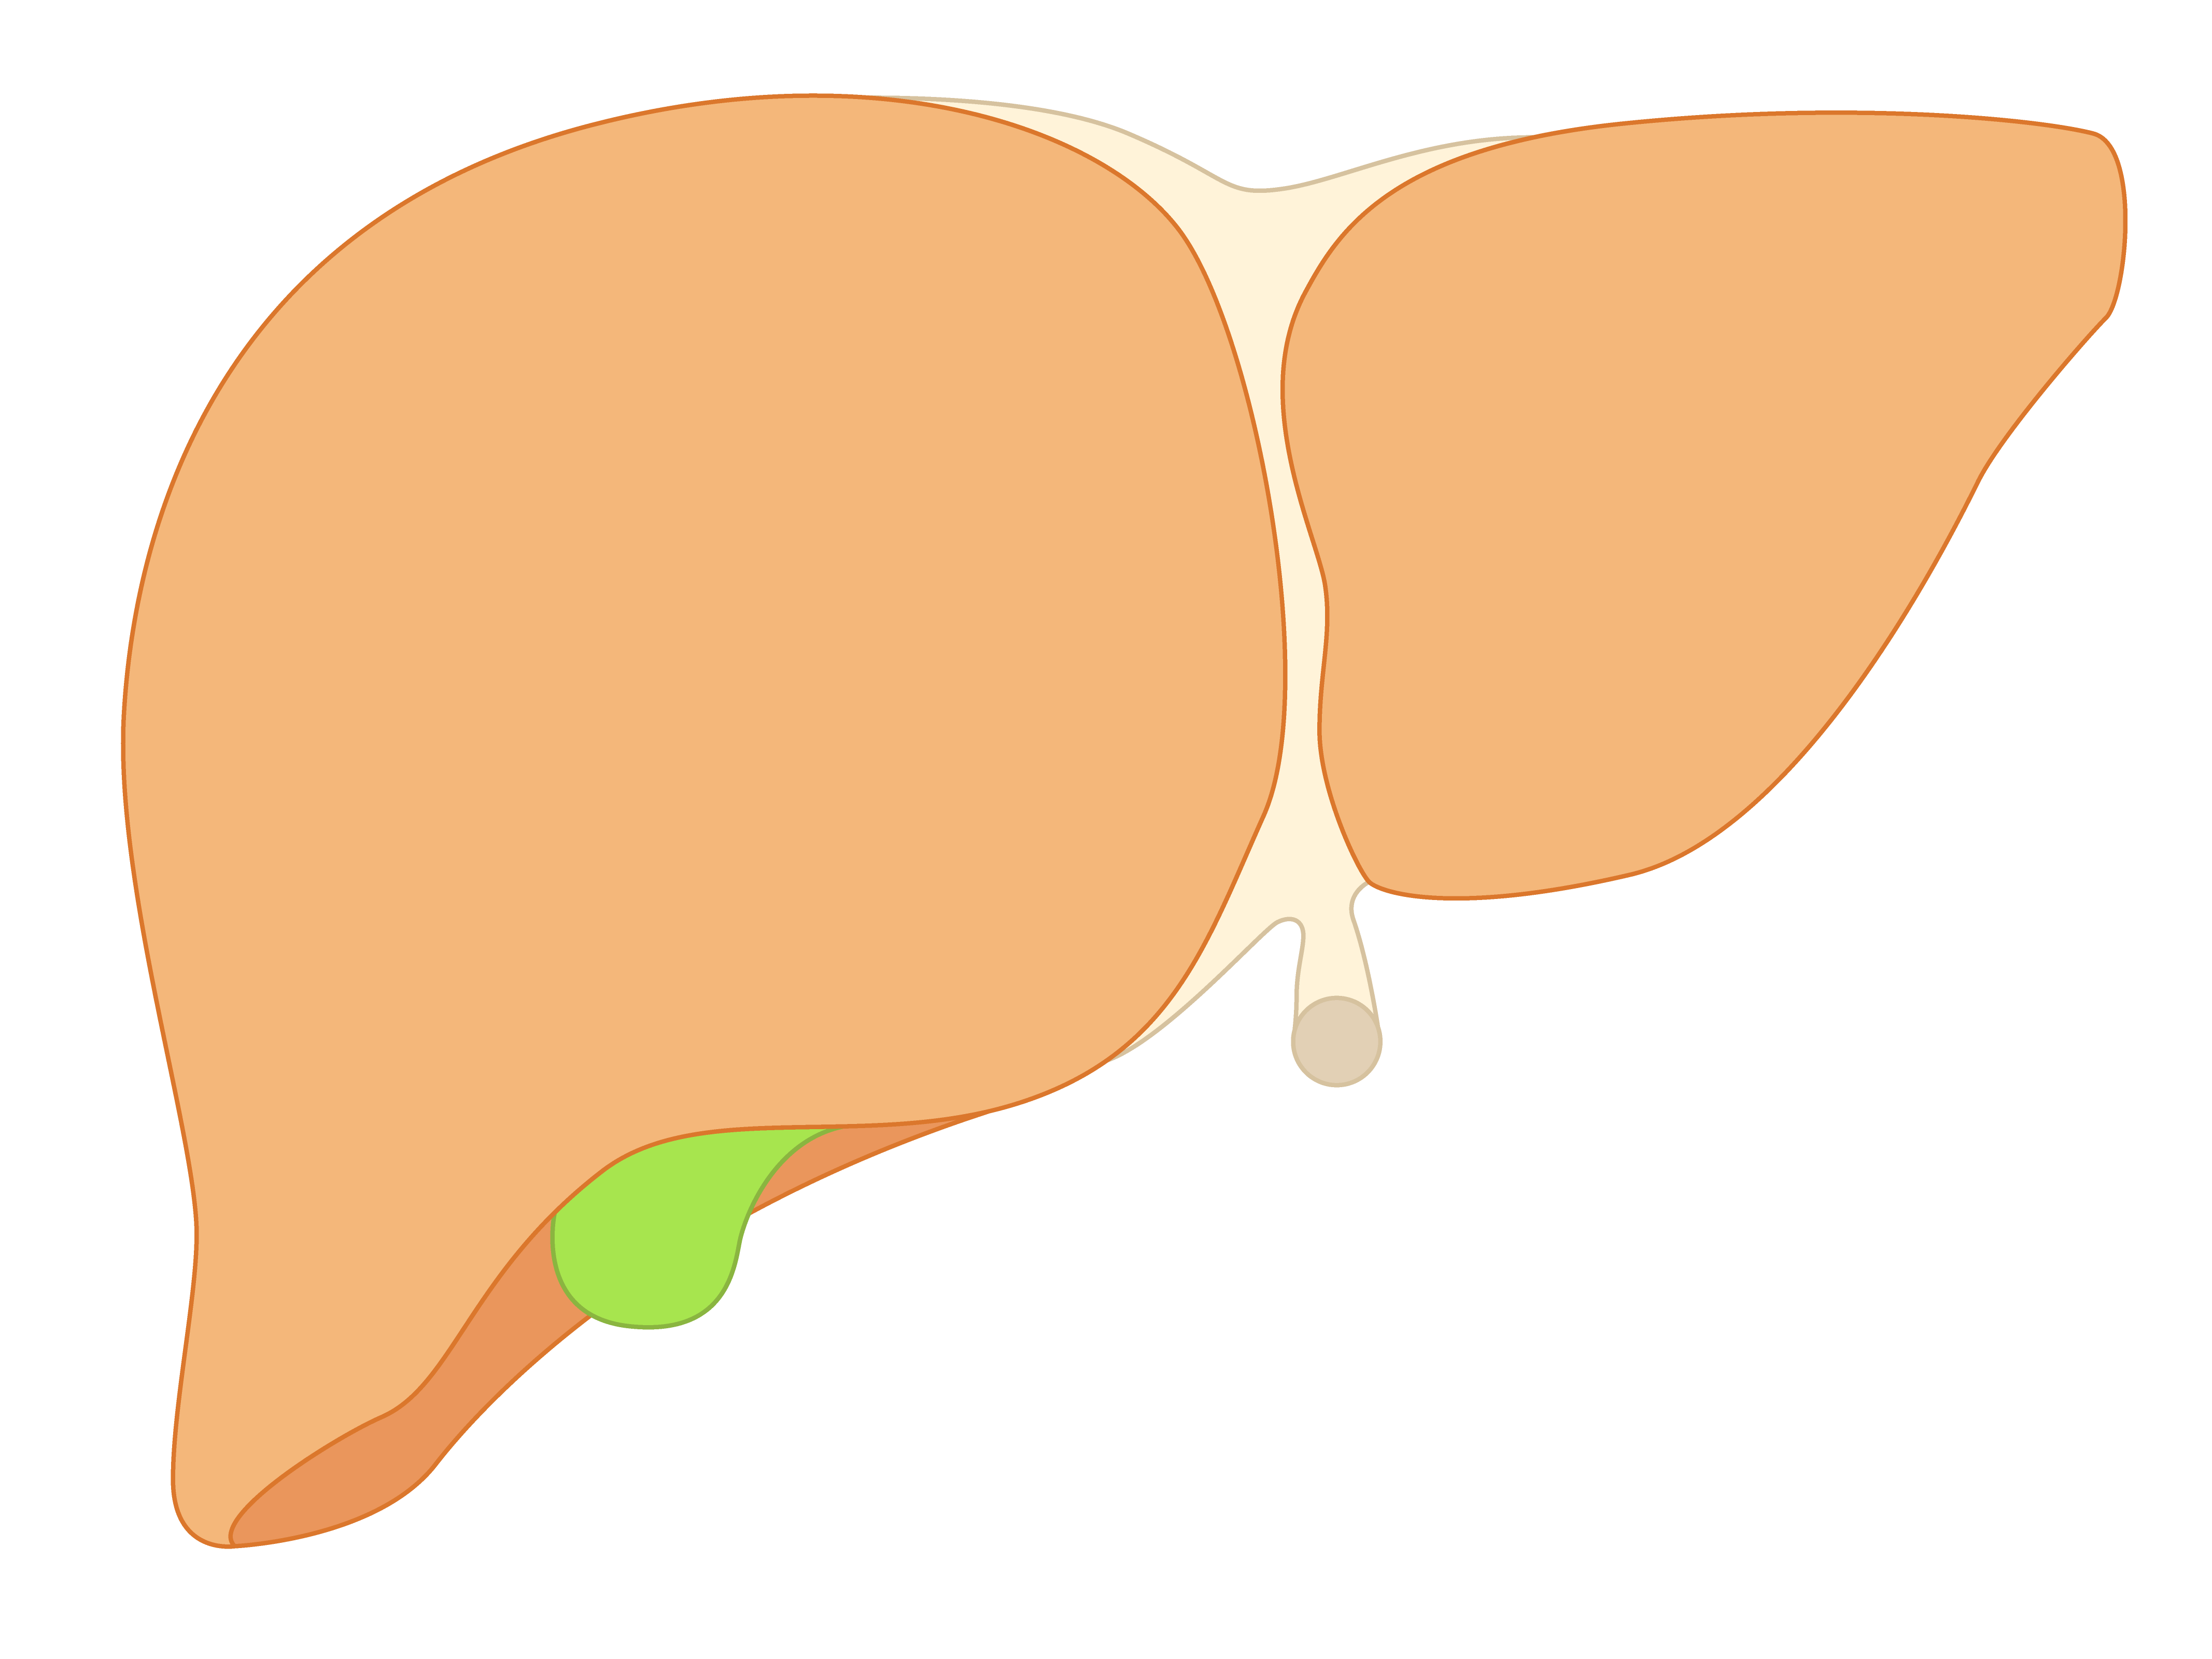
\includegraphics[width=\linewidth]{Figures/HealsyLiver.png}
  \caption{Схематичний зовнішній вигляд печінки}
  \label{fig:healthyliver}
\end{marginfigure}

\section{Де розташована печінка?}

Печінка знаходиться у правій верхній частині живота, під діафрагмою та захищена реберною дугою. 

\begin{marginfigure}[10pt]%
  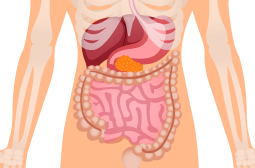
\includegraphics[width=\linewidth]{Figures/LiverRelation.png}
  \caption{Положення печінки в тілі людини}
  \label{fig:liverrelation}
\end{marginfigure}

Печінка розташована (Мал. \ref{fig:liverrelation}) поруч із шлунком, підшлунковою залозою, товстим кішківником, правою ниркою та наднирником і магістральними судинами організму — абдомінальними частинами аорти та нижньої порожнистої вени. \sidenote[][20pt]{Ця інформація важлива для розуміння принципу оперативного лікування новоутвореннь печінки, які виходять за межі органа}

\section{Яка внутрішня будова печінки?}

Печінка вкрай складний орган та має унікальну подвійну систему кровопостачання. Як і більшість органів в тілі людини, печінка отримує артеріальну кров з аорти по гілках печінкової артерії. Ця кров живить строму — каркас печінки, до якого входять жовчі протоки та судини в середині органа. Окрім того, на відміну від інших органів, печінка отримує по системі ворітної (портальної) вени ще й венозну кров від усіх непарних органів черевної порожнини, а саме шлунку, тонкого та товстого кішківника, селезінки та підшлункової залози (мал. \ref{fig:livervasculature}). Це дозволяє печінці переробляти поживні речовини, що всмоктуються в кров з кішківника під час процесу травлення. \sidenote[][10pt]{Розуміння кровопостачання печінки та системи портального кровотоку необхідне для усвідомлення принципу лікування пухлин печінки та портальної гіпертензії} 

Відтікає кров від печінки по системі печінкових вен, які впадають в нижню порожнисту вену поруч із правим передсердям. 


\newpage

\begin{figure*}[h]
  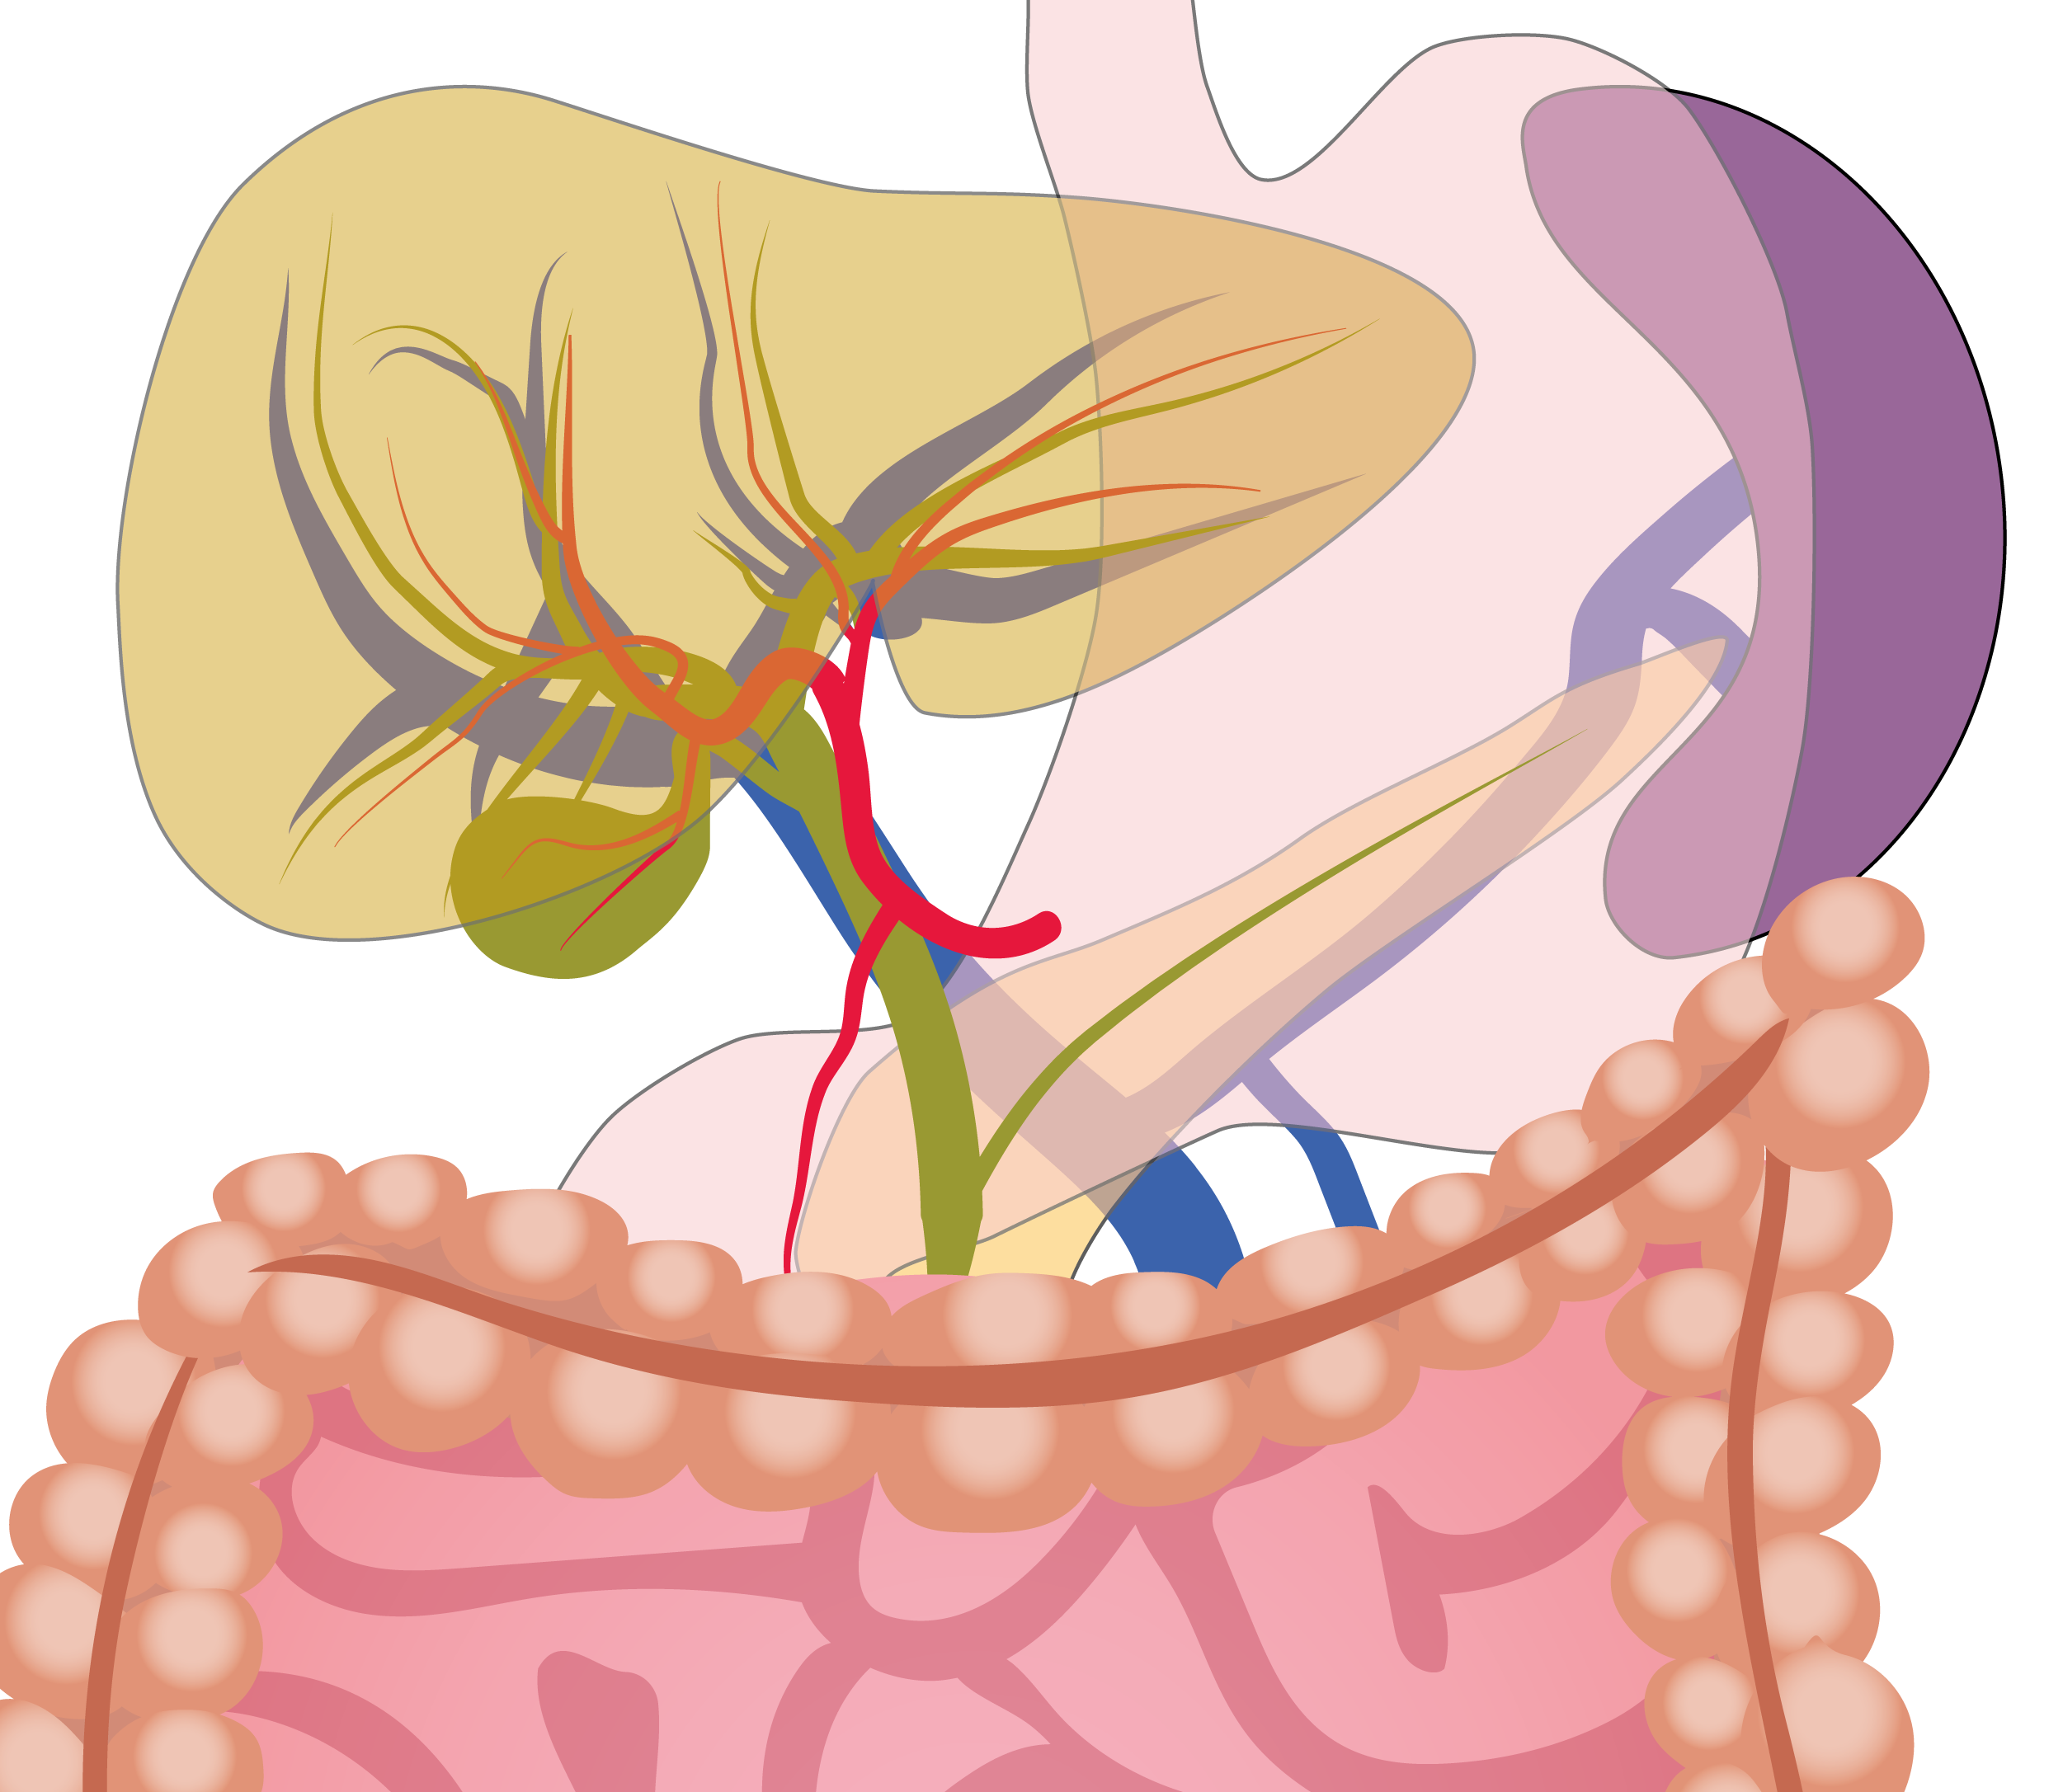
\includegraphics[width=\linewidth]{Figures/Liver vasculature_Liver and guts.png}%
  \caption{Кровопостачання печінки}%
  \label{fig:livervasculature}%
\end{figure*}

В середині печінки її судини та жовчні протоки поділяються, подібно до поділу стовбура дерева на гілки та утворюють судинно-секреторні пучки, що мають назву глісонових ніжок. Кожна з таких гілок (глісонова ніжка) має свою «крону листя» - окрему ділянку тканини печінки, яку вона кровопостачає та з якої відводить жовч.  Така ділянка тканини печінки має назву сегмент печінки (мал. \ref{fig:liversegments}). Всього печінка поділяється на вісім сегментів. 

\begin{marginfigure}%
  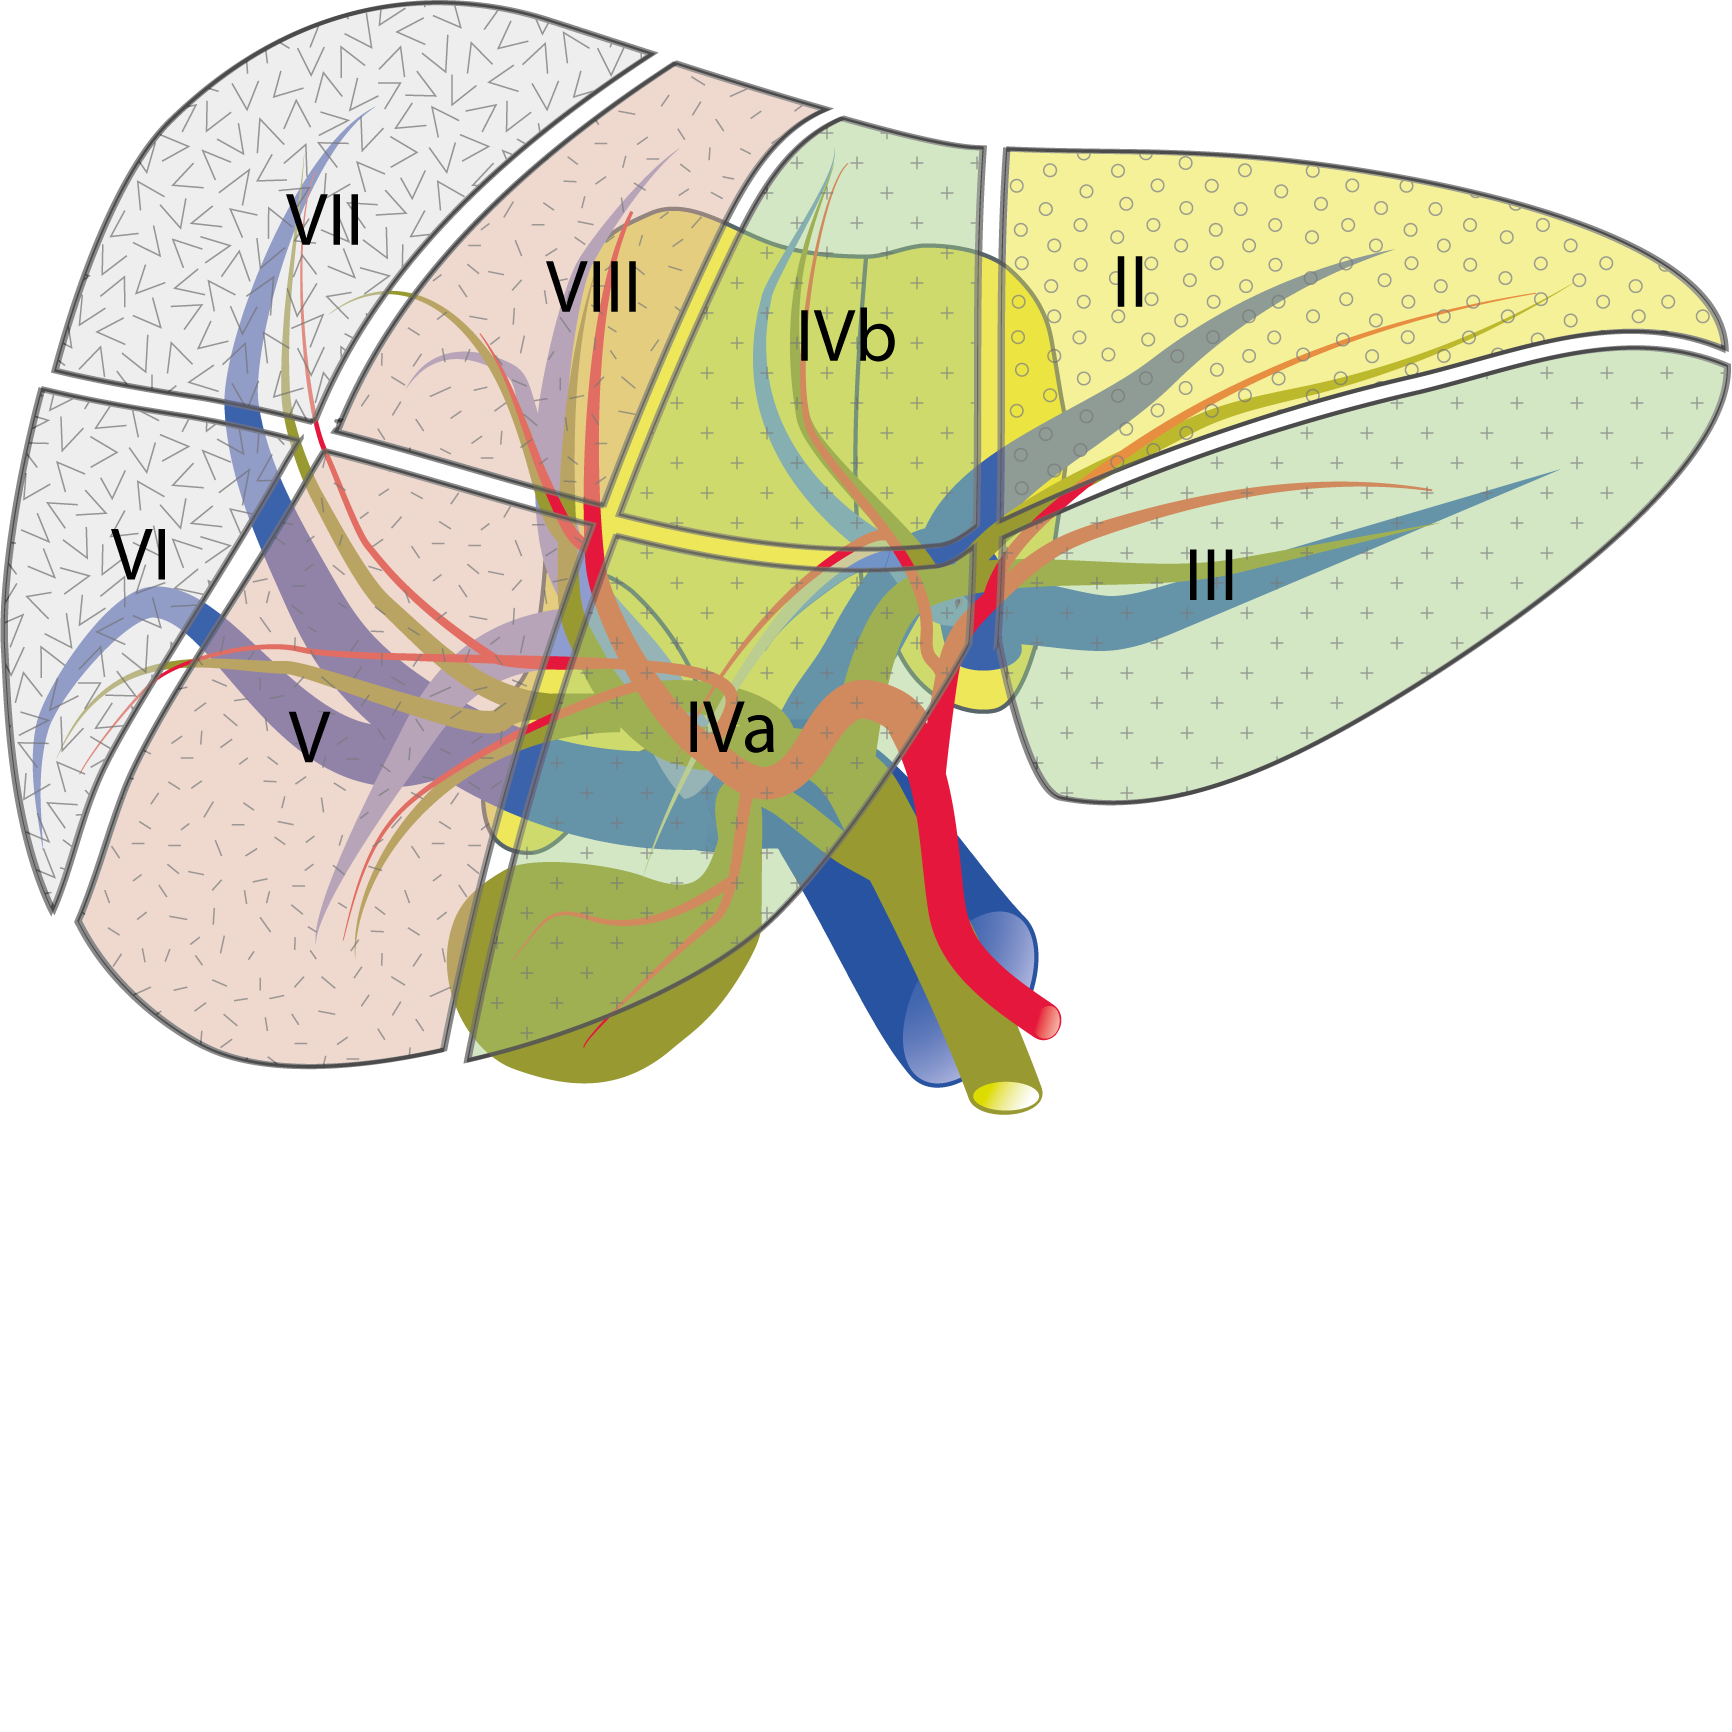
\includegraphics[width=\linewidth]{Figures/LiverSegments.png}
  \caption{Поділ печінки на сегменти}
  \label{fig:liversegments}
\end{marginfigure}

\begin{figure}
  \includegraphics[width=\linewidth]{Figures/Liver architecture-02.png}
  \caption{Гістологічна будова печінки. \par Тканина печінки складається з: а) паренхіми -- впорядкованих клітин печіни гепатоцитів та б) строми -- пучків судин та жовчних протоків}
  \label{fig:liverarchitecture}
\end{figure}

Сучасна хірургія печінки базується на видаленні новоутвореннь в межах окремих сегменітв печінки. Це більш безпечно, так як при цьому вся залишкова паренхіма має адекватне кровопостачання. Також це підвищує радикальність видалення пухлини.

\newpage
\section{Що таке жовч? Як вона виводиться?}

\begin{marginfigure}[-30pt]%
  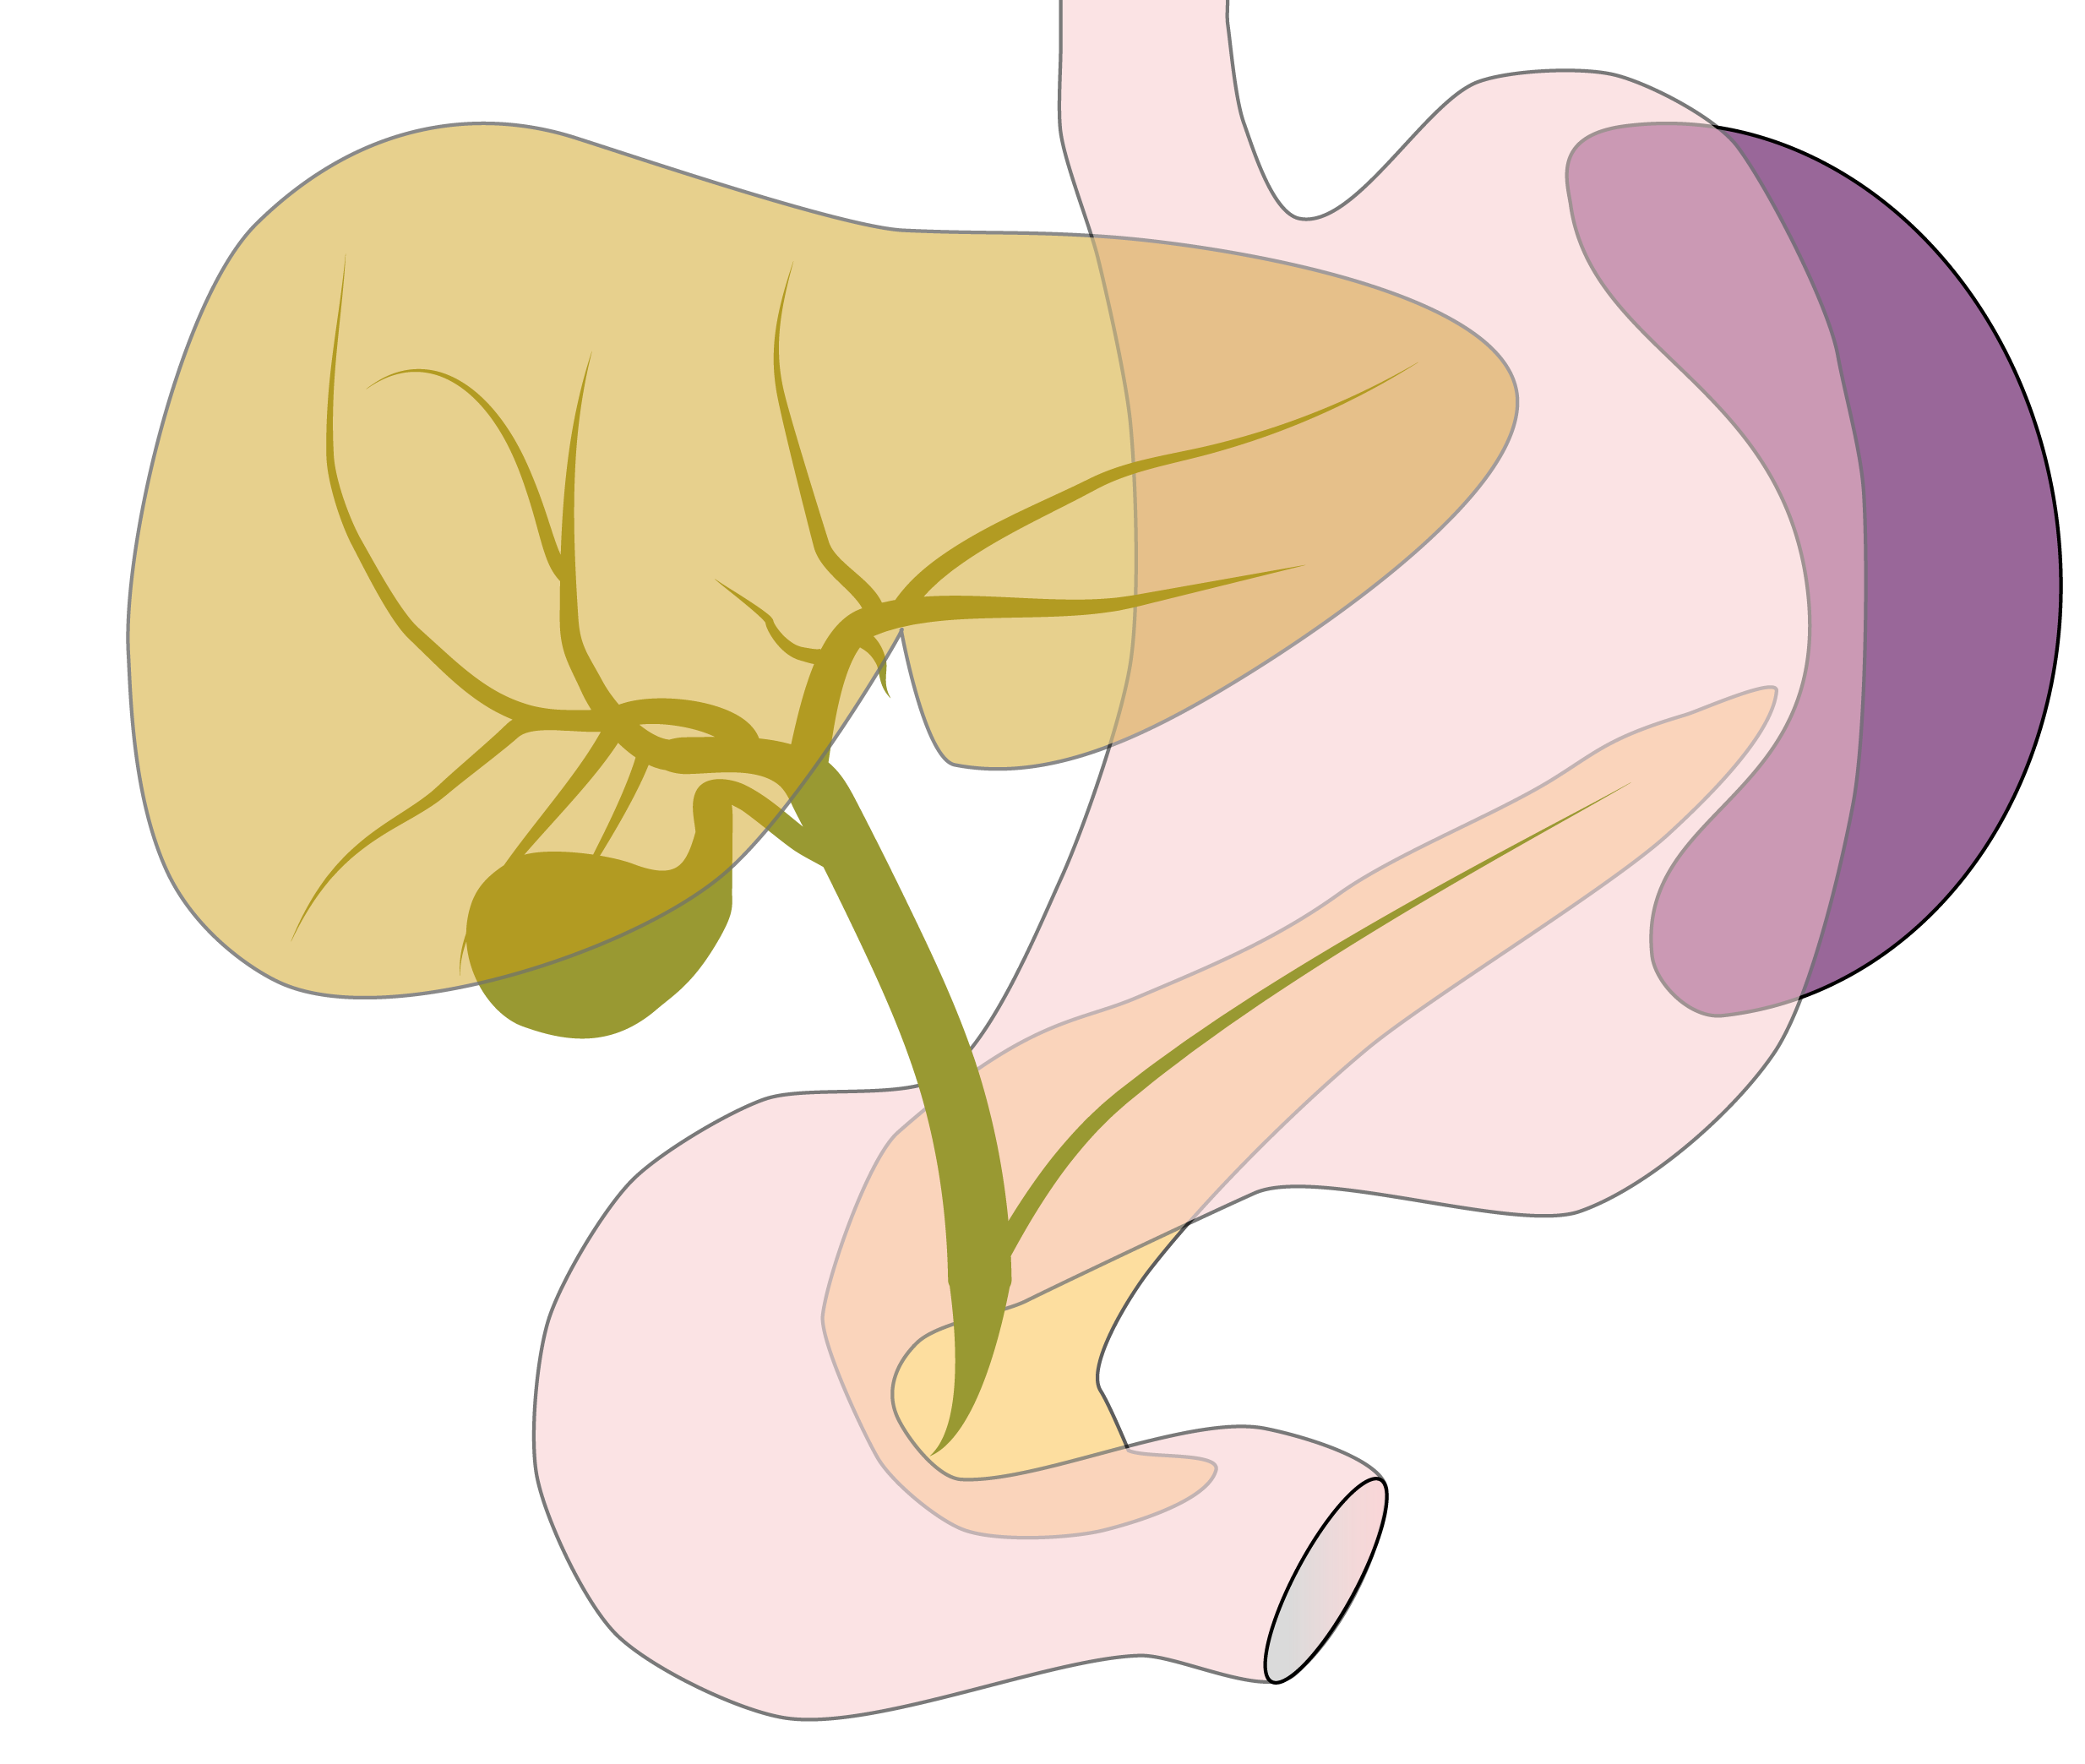
\includegraphics[width=\linewidth]{Figures/BileDucts_Focus on liver.png}
  \caption{Жовчні протоки печінки}
  \label{fig:bileducts}
\end{marginfigure}

Жовч — це необхідна для процесу травлення фізиологічна рідина, яку виділяють клітини печінки. По системі жовчних проток жовч потрапляє з печінки в кишківник.  Жовчні шляхи починаються в середині печінки у вигляді мікрокапелярів, потім об’єднуються та формують протоки все більшого діаметру. З печінки виходить одна велика протока, яка після об’єднання з протокою жовчного міхура, крізь тканину підшлункової залози потрапляє в дванадцятипалу кишку. \sidenote[][50pt]{Знання про систему жовчовідтоку необхідне для усвідомлення принципу лікування захворюваннь, що перебігають із механічною жовтяницею}


\section{Що таке жовчний міхур?}

Жовчний міхур це орган, який є частиною жовчовивідних шляхів. Жовчний міхур виконує функцію резервуара, де зберігається невелика кількість концентрованої жовчі між прийомами їжі. Після потрапляння їжі в травний канал жовчний міхур скорочується та викидає жовч в кишку, що полегшує травлення. Жовчний міхур не виробляє а лише зберігає малу частину жовчі (2-3\% від кількості яку печінка виділяє за добу). За його відсутності цю роль частково беруть на себе жовчні шляхи та печінка.

\begin{marginfigure}[50pt]%
  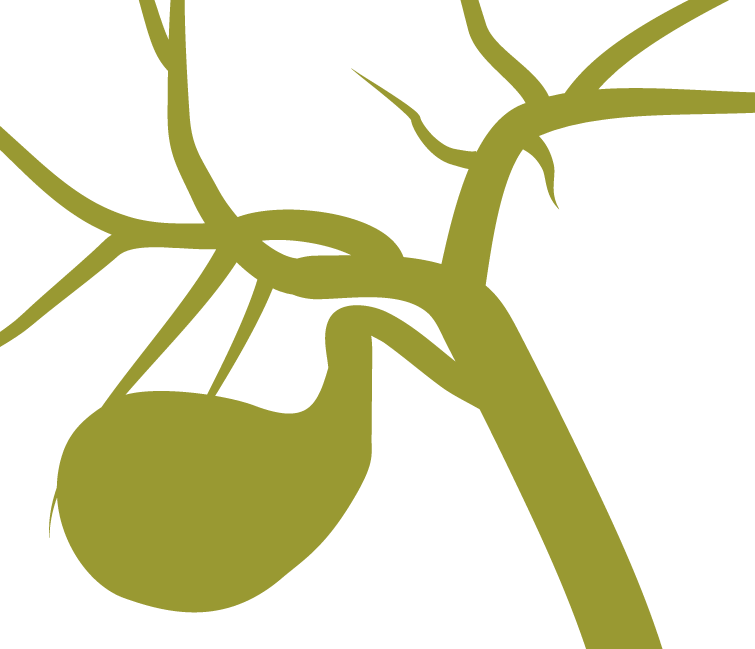
\includegraphics[width=\linewidth]{Figures/Goalbladder_Focus on hilum.png}
  \caption{Жовчий міхур - резервуар, який тимчасово зберігає невелику кількість жовчі}
  \label{fig:goalbladder}
\end{marginfigure}

\section{Які ще функції, окрім виділення жовчі, має печінка?}

Печінка - універсальна біохімічна лабораторія організму в якій відбувається метаболізм жирів, білків та вуглеводнів. Вона забезпечує організм енергією завдяки синтезу глюкози, яка є основною «енергетичною валютою».  Також  печінка зберігає запас глікогена - речовини, що за потреби швидко перетворюється на глюкозу. Печінка синтезує велику кількість білків плазми крові, таких, як альбумін та фактори згортання та деякі гормони. Також печінка є ключовим органом іммунної системи - вона є імунним бар’єром між портальною кров’ю з кішківника та системним кровотоком, а також тут синтезується 80-90\% імунних білків. Окрім цього, печінка відповідальна за знешкодження токсинів, які потрапляють в організм з їжею чи іншим шляхом. \sidenote[][30pt]{Інформація про печінкові функції та їх порушення необхідна для розуміння проявів її захворюваннь та/чи адекватної оцінки ризиків ускладненнь оперативного втручання}

\section{До чого призводить порушення функції печінки?}
Печінка є органом, що має велику здібність до регенерації та відновлення. Проте при вичерпанні цього ресурсу внаслідок захворювання функція її може порушуватись. \sidenote[][30pt]{Для визначення функціонального стану печінки найбільш часто використовують розширений біохімічний аналіз крові та коагулограмму. За результатами цих дослідженнь спеціаліст може зробити висновки про наявність чи відсутність порушення функції печінки. 

Окрім цього існує велика кількість спеціальних функціональних тестів, таких як  фіброеластографія, ICG-тест та ін. 

Про необхідність саме вам проходити той чи інший тест ви можете запитати у лікаря під час консультації}

Порушення функції печінки до таких проявів, як:
\begin{itemize}
  \item Жовтяниця - патологічний стан, при якому печінка не здатна захватити з крові та вивести із жовччю білірубін (токсичний пігмент, кінцевий продукт розпаду гемоглобіну), що призводить до пожовтіння всіх тканин організму та інтоксикації
  \item Порушення синтезу факторів згортання плазми, яке призводить до погіршання згортання крові та ризику спонтанних кровотеч та крововиливів
  \item Порушення синтезу альбуміну - головного білка-переносчика плазми крові, що призводить до зниження онкотичного тиску крові, набряклості тканей та продукції асциту (скупчення рідини в черевній порожнині)
  \item Печінкова енцефалопатія - ураження головного мозку токсинами кишкового походження через порушення їх знешкодження в печінці (сонливість, неуважність, роздратованість, дезорієнтованість та сповільнення темпу мови)
  \item Інфекції та септичні стани внаслідок ураження імунітету
\end{itemize}

\section{\LARGE{Що мені варто запам'ятати з цього розділу?}}



\begin{tcolorbox}[width=\textwidth,colback={YellowGreen},colbacktitle=yellow,coltitle=blue]    
\allcaps{Печінка - життєвоважливий орган, який має складну анатомічну будову та велику кількість необхідних для організма функцій.}
\end{tcolorbox}    
\begin{marginfigure}%
  
\includegraphics[width=\linewidth]{Figures/Exclamation_mark.png}
\end{marginfigure}
\begin{tcolorbox}[width=\textwidth,colback={Goldenrod},colbacktitle=yellow,coltitle=blue]   
\allcaps{Жовчний міхур є лише додатковою частиною жовчовивідних шляхів, яка відіграє допоміжну функцію в процесі виведення жовчі.}
\end{tcolorbox}    
